\section{Exact labels and admissible bounds}
The archived predecessor audit evaluates every stored nonnegative
state--goal label. Let $R$ be occupied blocker closure for required
removals and insertions. Without capacity or inspection obligations, the
formula $|A\triangle G|+2|R\cap A\cap G|$ agrees with all
\OldLabels{} audited labels. This is a finite-census equality, not a
general theorem about arbitrary assembly domains or visual perception.

For BrickPlan's lower bound, initially mismatched sites each require an
operation. Every occupied target site in the required removal closure
must be detached and reattached. Every unfinished job needs one audit.
These counts refer to disjoint required operations. Recursively including
occupied path blockers can only add necessary removals. Ignoring capacity
scheduling and some connectivity effects relaxes the problem, so
$h(x)\leq C^*(x)$. The verifier checks this inequality at every oracle node.

For every nonterminal product node, the certificate checks
$C^*(x)=\min_{a\in A(x)}[1+C^*(T(x,a))]$, with terminal cost zero.
Physical edges are compared with independent runtime transition
enumeration and inverse execution; audit edges are replayed as well.
Every retained product state reaches a terminal. The physical graph is
reversible within its capacity-constrained component. Audits add a
persistent bit without removing a physical action, and all admitted jobs
can be exposed. Consequently, legal successors do not become genuine
irreversible dead ends. Budget exhaustion and extra cost remain possible.

\section{Construction details}
The machine-readable source plan distinguishes development and
new-source groups before new-source solver discovery. Legacy tasks retain
their earlier selection bias. Additional task generation uses deterministic
seeds, sampled states and work orders, and solvability admission. Geometric
pruning was refined after an initial collision-rejecting pass, before
new-source policy results. Both passes and their exact retained source
indices are archived. No difficulty-based rejection is used for these
new-source tasks.

Ten geometry pairs share registered pieces and original transforms,
start, goal, capacity, jobs, and proposed action sequence. Induced fixed
contexts are separately qualified. Four context interventions across
source groups 31027, 10014, and 10036 yield these ten pairs, all with
unequal fixed-part counts. The remaining 37 qualified context candidates
yield no retained answer-changing pair under the declared search.
The full census is in
\texttt{data/geometry-probe-audit.json}.
Original/grayscale pairs preserve all geometry and labels.

The 144 interior-order pairs are balanced over conflict bins 2--5,
6--10, and 11+. Legal and reordered plans share exact prefixes up to
the first conflict, endpoints, and action multisets. Legal witnesses
have no repeated states. The stored audit exposes each conflict position,
so readers can run other prefix controls.

\begin{table}[t]
\centering\small
\caption{A prefix-only software control returns the first conflict if
it appears within $k$ executed operations, otherwise ``all legal.''
The denominator is all 288 continuation questions.}
\begin{tabular}{rrr}\toprule
Prefix length & Correct / assigned & Accuracy\\\midrule
0 & 144/288 & 50.0\%\\
1 & 144/288 & 50.0\%\\
2 & 158/288 & 54.9\%\\
3 & 172/288 & 59.7\%\\
5 & 192/288 & 66.7\%\\
8 & 224/288 & 77.8\%\\
11 & 248/288 & 86.1\%\\
16 & 273/288 & 94.8\%\\
24 & 282/288 & 97.9\%\\
32 & 288/288 & 100.0\%\\
\bottomrule\end{tabular}

\end{table}

\section{Shallow choice and control diagnostics}
\begin{table}[t]
\centering\small
\caption{Measured finite-horizon choice sets for all 653 next-action
questions. Any/all refer to optimistic/pessimistic ties; uniform tie
correctness is an exact average, not a sampled policy result.}
\resizebox{\columnwidth}{!}{\begin{tabular}{rrrrr}\toprule
Depth & Choices & All optimal & Any optimal & Uniform tie\\\midrule
1 & 653 & 571 & 653 & 94.0\%\\
2 & 653 & 592 & 653 & 95.4\%\\
4 & 653 & 590 & 653 & 94.7\%\\
8 & 653 & 612 & 653 & 96.6\%\\
\bottomrule\end{tabular}
}
\end{table}
The depth-one minimizing set contains an optimal action at all 653
selected checkpoints. Therefore the diagnostic bank does not demonstrate
that shallow reasoning necessarily excludes the correct answer.
Deeper horizons can change tie composition nonmonotonically. The full
table is retained without redefining difficulty to match its results.

\begin{table}[t]
\centering\small
\caption{Structural policy completion by operation-length bin.
Each nonoracle policy has three tie-order seeds per episode.}
\resizebox{\columnwidth}{!}{\begin{tabular}{lrrrr}\toprule
Control & D1 & D2 & D3 & D4\\\midrule
Closure greedy & 291/291 & 449/456 & 242/249 & 79/135\\
Capacity dispatch & 291/291 & 450/456 & 232/249 & 66/135\\
Closure A* (100) & 291/291 & 447/456 & 225/249 & 45/135\\
Closure A* (1,000) & 291/291 & 456/456 & 240/249 & 92/135\\
Closure A* (full) & 291/291 & 456/456 & 249/249 & 135/135\\
Hamming A* (full) & 291/291 & 456/456 & 249/249 & 135/135\\
\bottomrule\end{tabular}
}
\end{table}
All \RawPolicyRuns{} raw policy task-run records are archived in
\texttt{data/software-control-records.json.gz}. They include one oracle
seed and three seeds for nine other policies, with actions, outcomes,
expansions, timings, and regrets. The release checker recomputes every
overall, tier, source, and seed aggregate. The full search cap of
500,000 is a resource ceiling, not actual expansion usage. Oracle loading
and cached local timing are not comparable to calibrated online search.

\section{Recovery, diagnosis, and censoring}
Traverse only edges with $C^*(T(x,a))=C^*(x)-1$ from pre-error state
$b$. The reached states are exactly the union of optimal completions:
each traversal is an optimal prefix, and every optimal prefix satisfies
that equality. Remove the terminal state to obtain the repair target
$\mathcal C_b^{-}$. The generator's delayed checkpoints remain outside
this set after an error and lag 1, 3, or 5. Independent forward BFS
verifies their shortest return distances, which range from 1 to 7.
The 943 questions comprise 337, 307, and 299 checkpoints at those lags.

Each positive-excess legal action creates its own spontaneous event;
later actions update every active event. A second error never replaces
the first. Immediate recovery and lag-specific delayed cohorts are
reported separately. Unfinished events are censored; terminal events
that never restore a nonterminal corridor state are observed failures.
Reaching a goal after a costly detour earns completion credit, but not
automatic corridor-repair credit.

The inverse-last-action control uses only the public executed history
and candidate list. It earns zero when no inverse is offered. It solves
235/337 lag-one, 162/307 lag-three, and 150/299 lag-five questions.
The combined 547/943 accuracy is 58.0\%. There are 368 cases with a legal
but suboptimal inverse and 28 with no offered inverse. Lag is thus an
experimental descriptor, not proof of necessary nonlocal reasoning.

There are 26 all-correct-choice calibration questions across the
diagnostic bank. Their correct tie sets are preserved, and the evaluator
reports calibration separately from the 1,926 discriminative rows.
The 1,952 rows map to 1,819 canonical problems. Assigned repeated variants
are averaged before problems and sources; missing responses receive
zero before this averaging. The evaluator exposes both row and clustered
scores, plus each inverse-control cohort. None of these private labels
is included in the policy observation.

An accepted diagnosis concerns legal positive-excess events since the
last diagnosis or episode start. The first later diagnosis is attached
to each previously undiagnosed event, with its sign and lag. True
positive diagnosis checkpoints open replanning-suffix records.
Always-negative or selectively requested diagnoses can yield misleading
accuracy, so report event detection and query coverage alongside it.

Plan-survival reports retain the first cost loss even after recovery,
and include explicit eligible/observed/unknown counts per operation index.
They are descriptive task-budget curves, not Kaplan--Meier population
estimates. Conditions should use matched assignments and registered
source strata. Missing episodes must not disappear from denominators.

\subsection{Regret conservation}
For a successful trace, accepted attaches $A_c$ and detaches $D_c$
satisfy $A_c-D_c=\Delta$, the target-minus-start occupancy count.
There are exactly $u$ accepted previously unfinished audits.
Duplicate audits are rejected. If $N_{\rm invalid}$ is the number of
charged invalid attempts, then
\begin{align}
T &=2D_c+\Delta+u+N_{\rm invalid},\\
C^*(x_0)&=2D^*+\Delta+u,\\
T-C^*(x_0)&=2(D_c-D^*)+N_{\rm invalid}.
\end{align}
This audit-inclusive identity reconciles detachment regret and total
excess. Rejected actions consume budget; stale HTTP revisions and malformed
request envelopes are rejected before mutation and are not action events.

\begin{table*}[t]
\centering\small
\caption{Metric denominators and treatment of missing outcomes.}
\begin{tabular}{p{.22\textwidth}p{.38\textwidth}p{.30\textwidth}}\toprule
Metric & Eligible denominator & Missing / termination rule\\\midrule
Completion / optimal completion & All assigned episodes & Unstarted and unfinished are failures\\
Successful mean regret & Successfully finished episodes & Null for failures; report success coverage\\
Avoidable-cost choice & Legal decisions with zero- and positive-excess alternatives & Invalid attempts excluded here, charged in total\\
Budget-loss choice & Viable checkpoints with viable and nonviable legal choices & Other budget losses remain in raw records\\
True-unreachability choice & No eligible choices in retained components & Undefined, not empirical evidence of zero risk\\
Recovery bounds & Every eligible legal positive-excess event & Lower bound restored/all; upper adds censored\\
Diagnosis accuracy & Accepted diagnosis queries & Unqueried intervals are not inferred correct\\
Joint pair correctness & Fully assigned pairs & Missing member prevents joint credit\\
Discriminative probe accuracy & Assigned noncalibration questions of that family & Missing or invalid response gets no credit\\
Source macro accuracy & Variants within problem, then problems within source, then sources & Missing variants enter as zero before averaging\\
Calibration accuracy & Assigned all-correct-choice questions & Report separately; not evidence of discrimination\\
\bottomrule\end{tabular}
\end{table*}

\section{Visual stimuli and actual model calls}
All executable geometry uses original source poses and LDraw triangle
meshes. The 214 distinct part meshes contain 290,338 triangles.
\texttt{ASSET-LICENSES.json} preserves source models, authors, URLs, and
part-level notices; attribution and licenses remain separate from code.
Qualification proxies do not replace the displayed shapes.
Figure provenance records exact states, seeds, bank hash, and image hashes.

The public renderer supersamples by two before Lanczos downsampling to
native HD. Display canvases account for device-pixel ratio, and native
zoom avoids CSS-only enlargement of low-resolution pixels.
Catalog tiles are $480\times360$ and catalogs are 1920 pixels wide.
Models receive image content, not text describing images. Preprocessing
is separately declared: the local SmolVLM case resizes to longest edge
512, with splitting disabled. HD display does not imply native-HD model
processing.

The preserved version-2.1 local case contains four actual inference calls
on historical public E069, seed 0. The original task and bank hash are
archived; this trace is not relabeled as version-2.2 evaluation.
All calls return descriptive prose instead of an executable JSON action.
The executor rejects each, and the controller stops at its four-call limit.
Every prompt, raw response, image hash, latency, measured token count,
action, and feedback is archived. No oracle action or fabricated explanation
replaces model output. This is a failed integration example. It supplies
neither an estimate of SmolVLM accuracy nor evidence about larger VLMs.

\section{Protocol and reproducibility}
Study runs bind participant, condition, seed, assignments, and bank hash.
The evaluator replays mutations, validates views, and normalizes candidate
permutations. Retries are idempotent across restart; changed content or
stale revisions are rejected. Failed atomic persistence rolls back mutations.

Practice exposes rich catalogs, solution review after submission, and
free 3D inspection. Study mode blocks these and private downloads.
Portable evaluator data must remain on the evaluator host during blind
studies; a local working-directory convention is not a security sandbox.

The practice model manager supports local MLX and OpenAI-compatible
vision calls, durable outputs, and bounded run/step/stop. Credentials
never enter browser exports. Stop prevents subsequent actions, not
in-flight provider billing. Interrupted calls are never silently retried.

The population study runner is distinct. Its reported-usage mode reserves
maximum tokens and cost before calls; adapters account for images and
attest usage. Missing accounting, timeout, malformed responses, or limit
violations stop continuation. Unavailable-accounting mode marks tokens
and currency unavailable. This relies on adapter/provider reports, not
a provider-enforced spending quota.

The main paper uses the unmodified official CVPR author-kit, pinned to
commit \texttt{2917585}, labeled 2026. A future year's kit is not claimed.
The PDF uses public preprint mode without margin/font compression.
Review mode requires the actual year and paper ID.

\clearpage
\onecolumn
\section{Base source assemblies}
The table lists 17 base assemblies from 16 kit groups; roadster and kart
share kit 31027. An additional 82 qualified context profiles are indexed
in the machine-readable source census. They are not independent sources.
Profiles without episodes are zero-yield candidates, not benchmark tasks.
Registered and movable counts describe different quantities.
\begin{center}\small
\begin{tabular}{llrrrr}\toprule
Base assembly & Kit & Parts & Registered & Movable & Episodes\\\midrule
Roadster body & 31027 & 37 & 17 & 17 & 14\\
Kart deck & 31027 & 25 & 18 & 18 & 14\\
Airframe & 31028 & 24 & 21 & 21 & 14\\
Truck cab and roof & 10156 & 76 & 18 & 18 & 10\\
House roof assembly & 31009 & 221 & 18 & 17 & 14\\
Sports car upper body & 5867 & 149 & 22 & 10 & 3\\
Source 10001 subassembly & 10001 & 17 & 2 & 2 & 8\\
Source 10159 subassembly & 10159 & 177 & 16 & 16 & 12\\
Source 10220 subassembly & 10220 & 153 & 16 & 16 & 12\\
Source 10014 subassembly & 10014 & 71 & 16 & 15 & 12\\
Source 10128 subassembly & 10128 & 98 & 16 & 14 & 12\\
Source omr-31031 subassembly & 31031 & 42 & 12 & 12 & 12\\
Source 10036 subassembly & 10036 & 79 & 16 & 16 & 48\\
Source 10213 subassembly & 10213 & 179 & 2 & 2 & 28\\
Source omr-10242 subassembly & 10242 & 180 & 16 & 16 & 48\\
Source omr-10265 subassembly & 10265 & 179 & 4 & 4 & 48\\
Source omr-10269 subassembly & 10269 & 105 & 16 & 11 & 48\\
\bottomrule\end{tabular}

\end{center}
\begin{center}\small
\begin{tabular}{lrrrr}\toprule
Partition & Sources & Episodes & Greedy & Full A*\\\midrule
Development & 8 & 109 & 87.2\% & 100.0\%\\
Held-out source & 8 & 268 & 96.5\% & 100.0\%\\
\bottomrule\end{tabular}

\end{center}
Version 2.2 admitted five of eleven additional frozen source candidates.
The other six remain in the source-plan rejection census. Only source
geometry and solvability determine this admission; no policy-performance
threshold is used. All earlier episode and diagnostic definitions are
preserved. New annotations specify scoring roles and canonical identities.

\section{Static and active view certificates}
Static diagnostics supply four fixed views at revision zero: isometric,
left, rear, and right. All five panels are included for each view, and
later acquisition is disabled. The structured diagnostic condition uses
the same initial views. Active image diagnostics begin with isometric
only; each inspect increments the view budget. These are separate
conditions rather than interchangeable names for one observation.

The native-resolution certificate compares every geometry pair in all
twenty initial panels. All ten pairs have at least one pixel-distinct
view; three pairs have identical isometric panels. The certificate is
bound to the bank hash and identity seed. It demonstrates input
distinguishability, not human agreement or perceptual answerability.
Other image-processing pipelines and identity seeds require their own
checks. Study results must report preprocessing and acquisition counts.
\clearpage
\section{Original-source gallery: assemblies 1--6}
\begin{center}
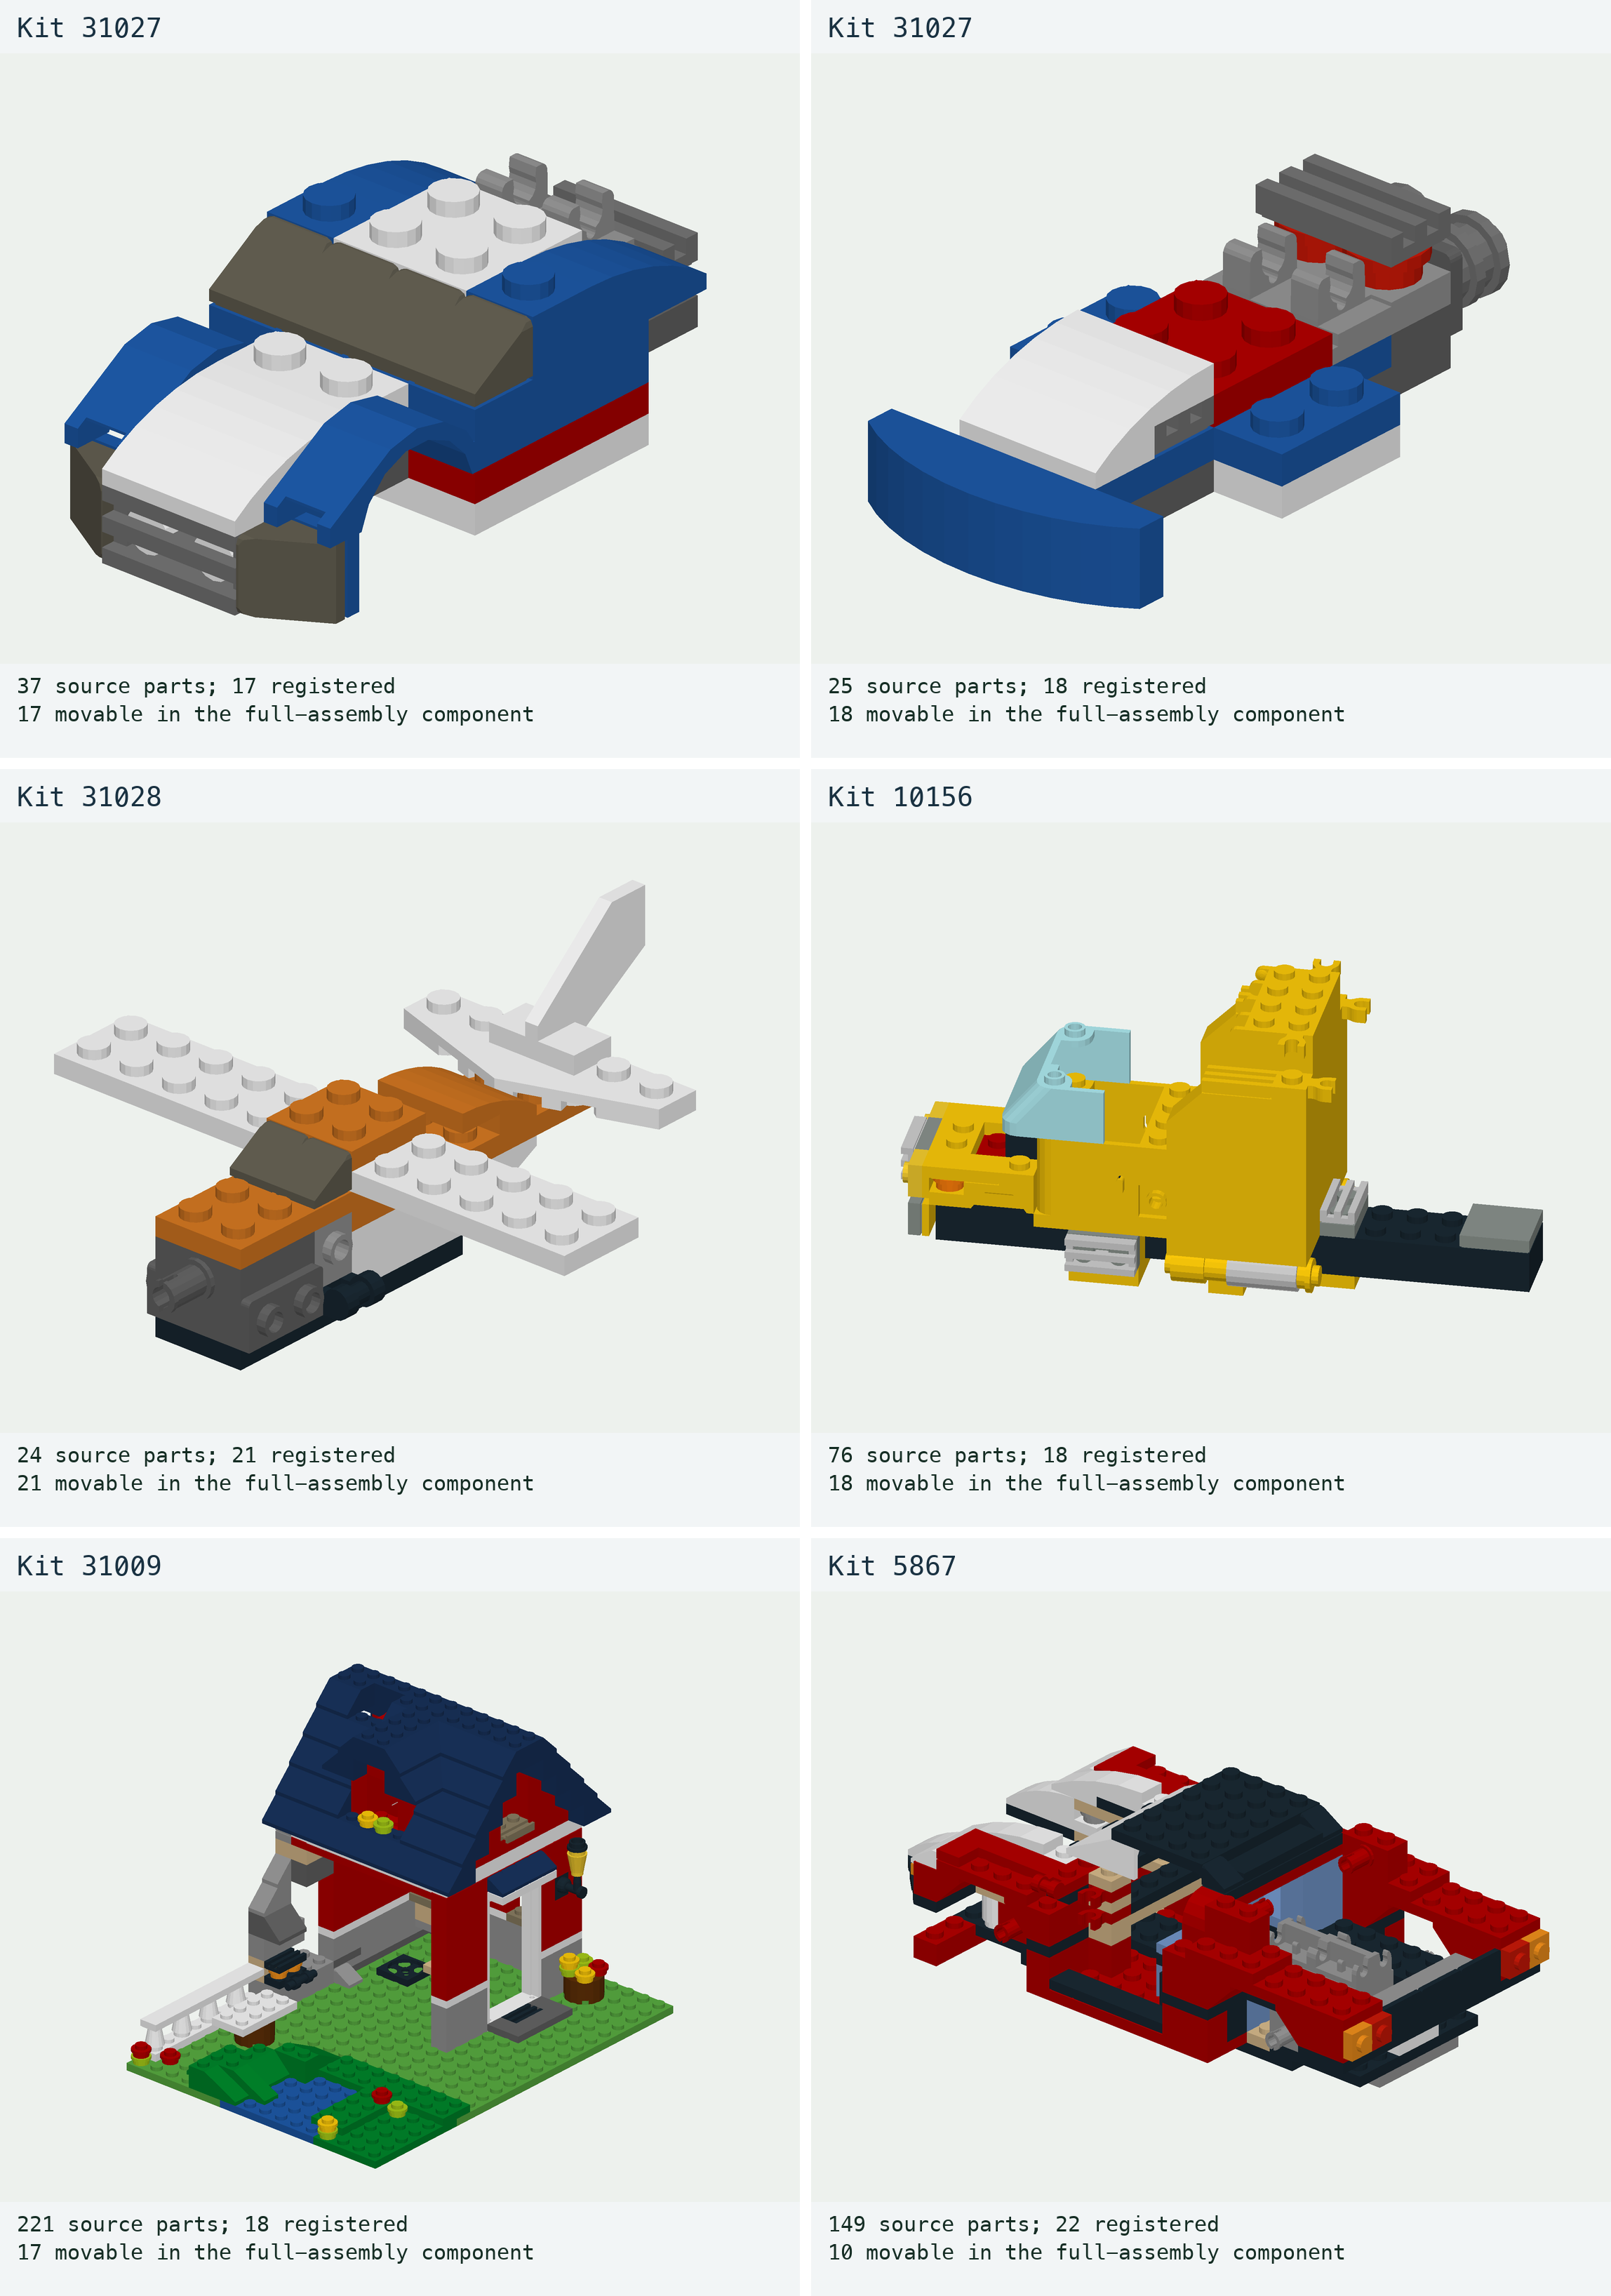
\includegraphics[width=.96\textwidth,height=.85\textheight,keepaspectratio]{figures/source-gallery-1.png}
\end{center}
\clearpage
\section{Original-source gallery: assemblies 7--12}
\begin{center}
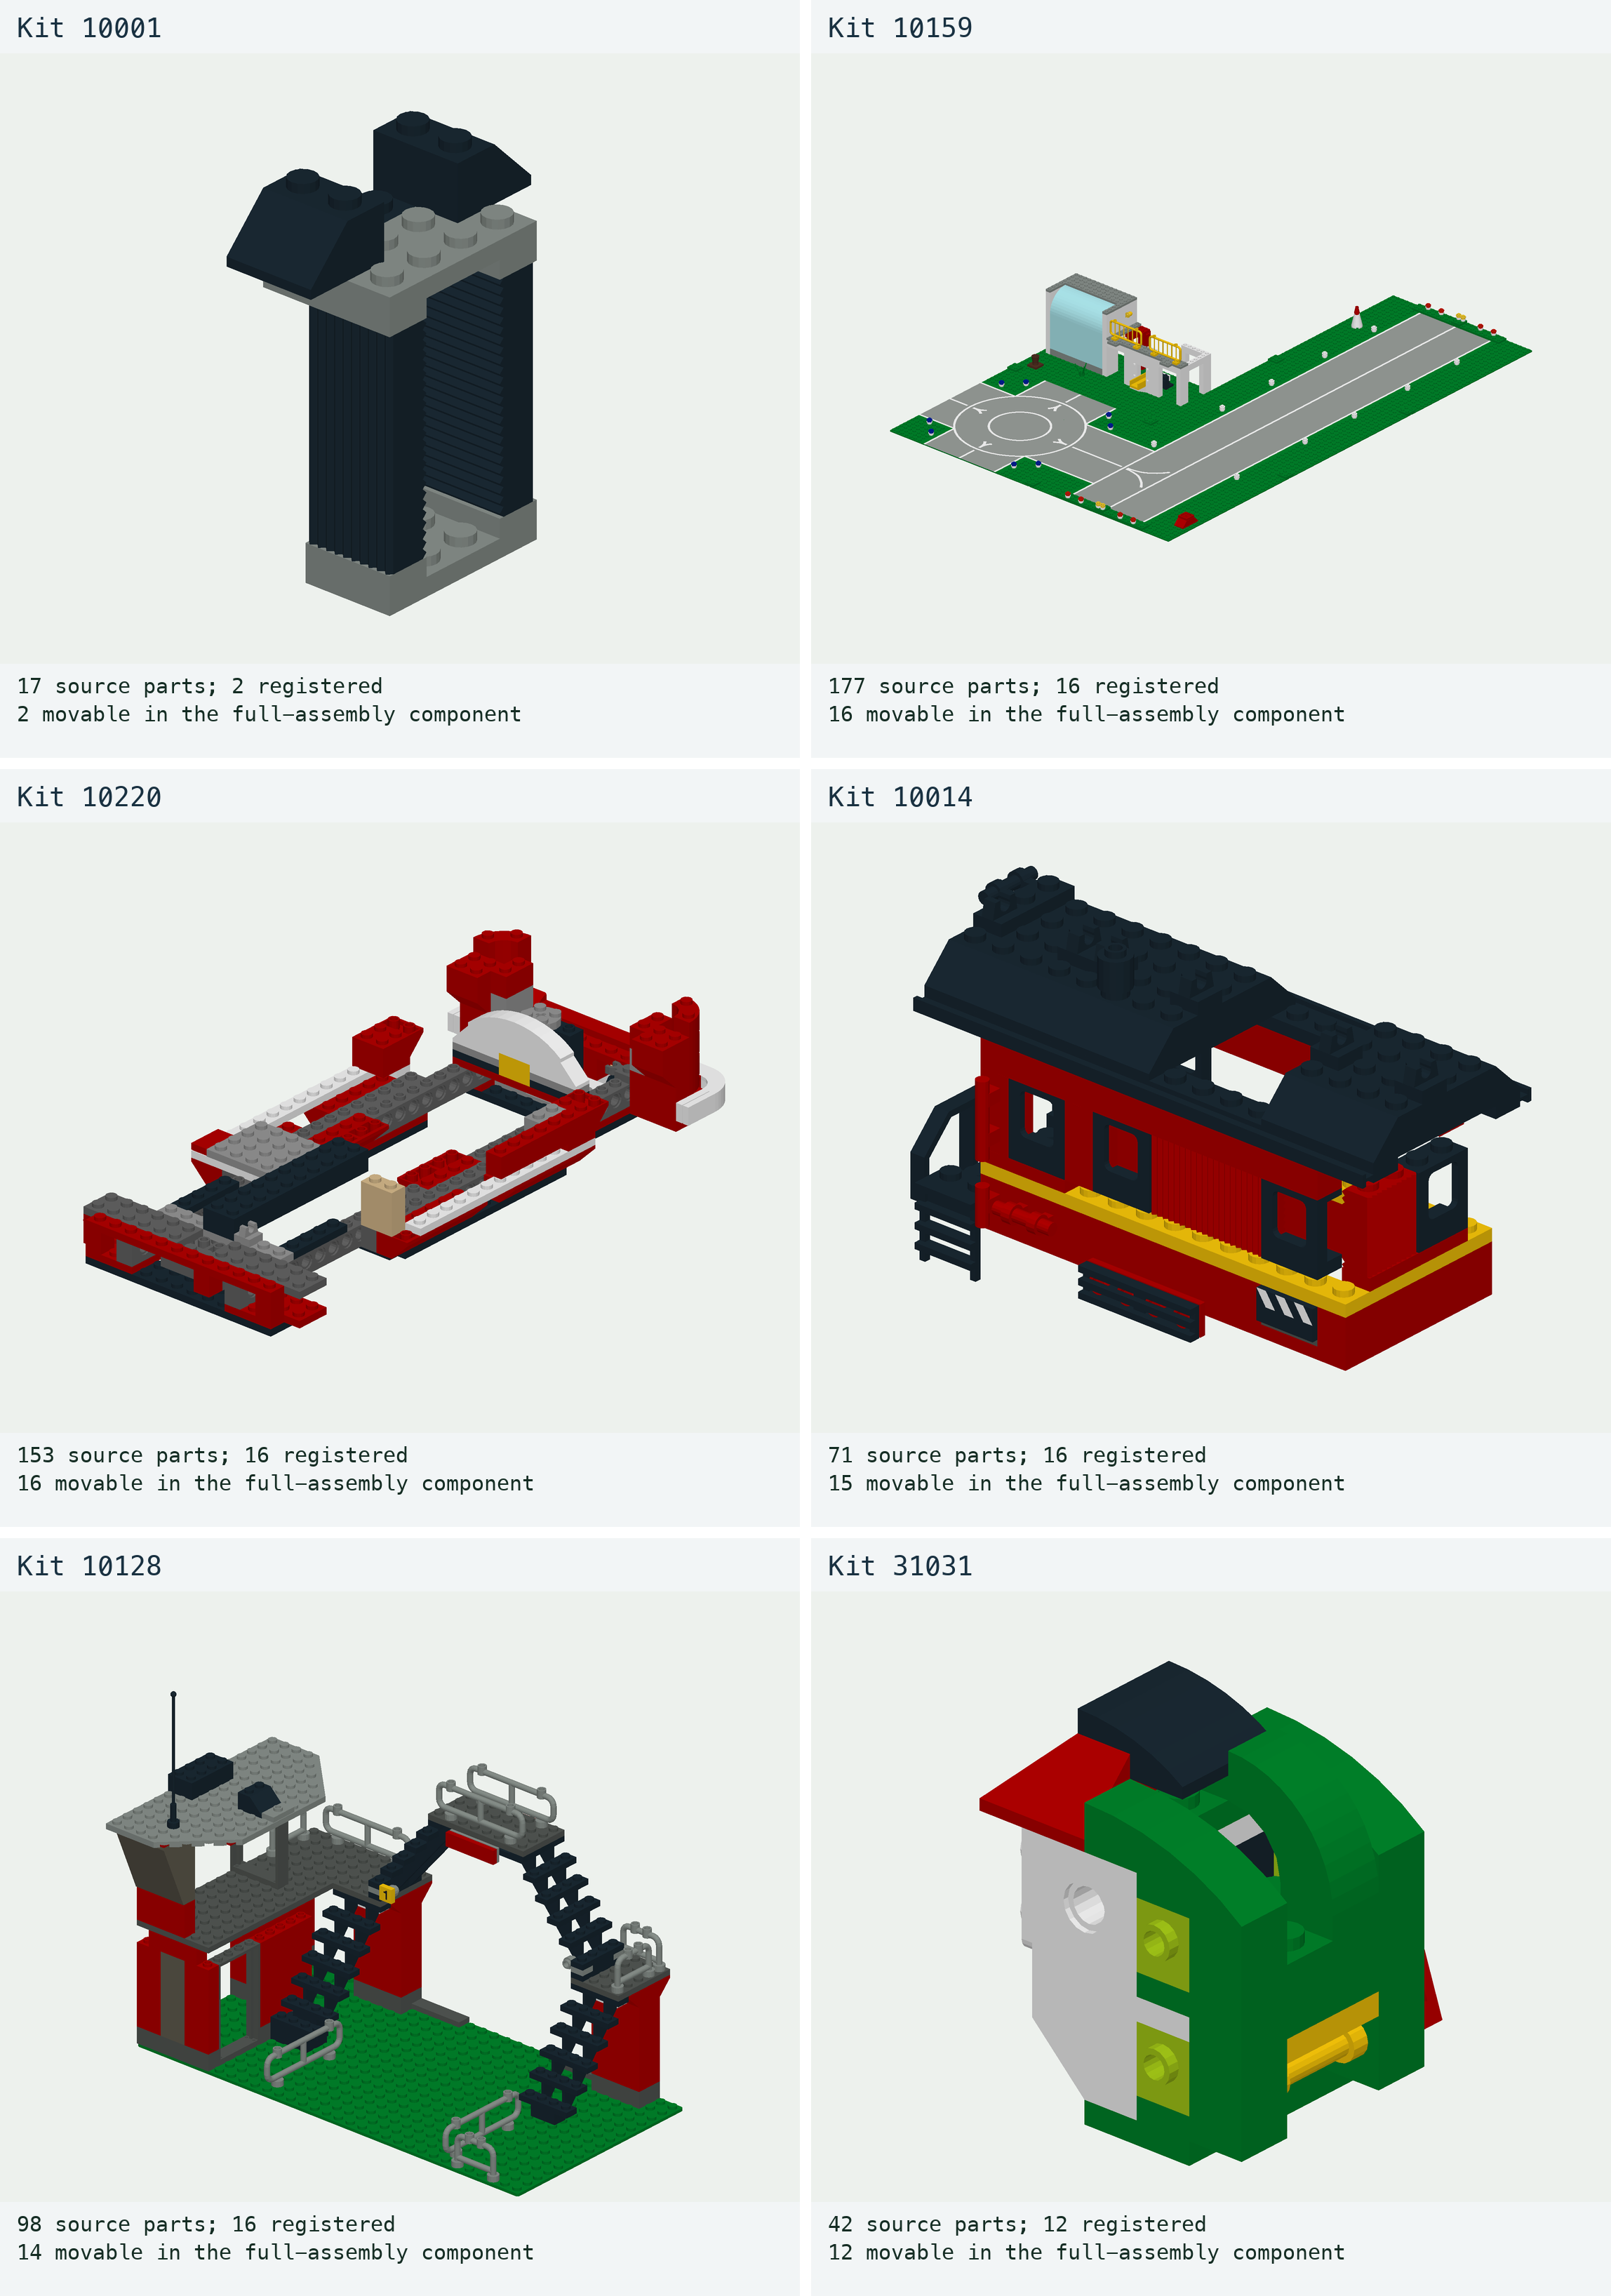
\includegraphics[width=.96\textwidth,height=.85\textheight,keepaspectratio]{figures/source-gallery-2.png}
\end{center}
\clearpage
\section{Original-source gallery: assemblies 13--17}
\begin{center}
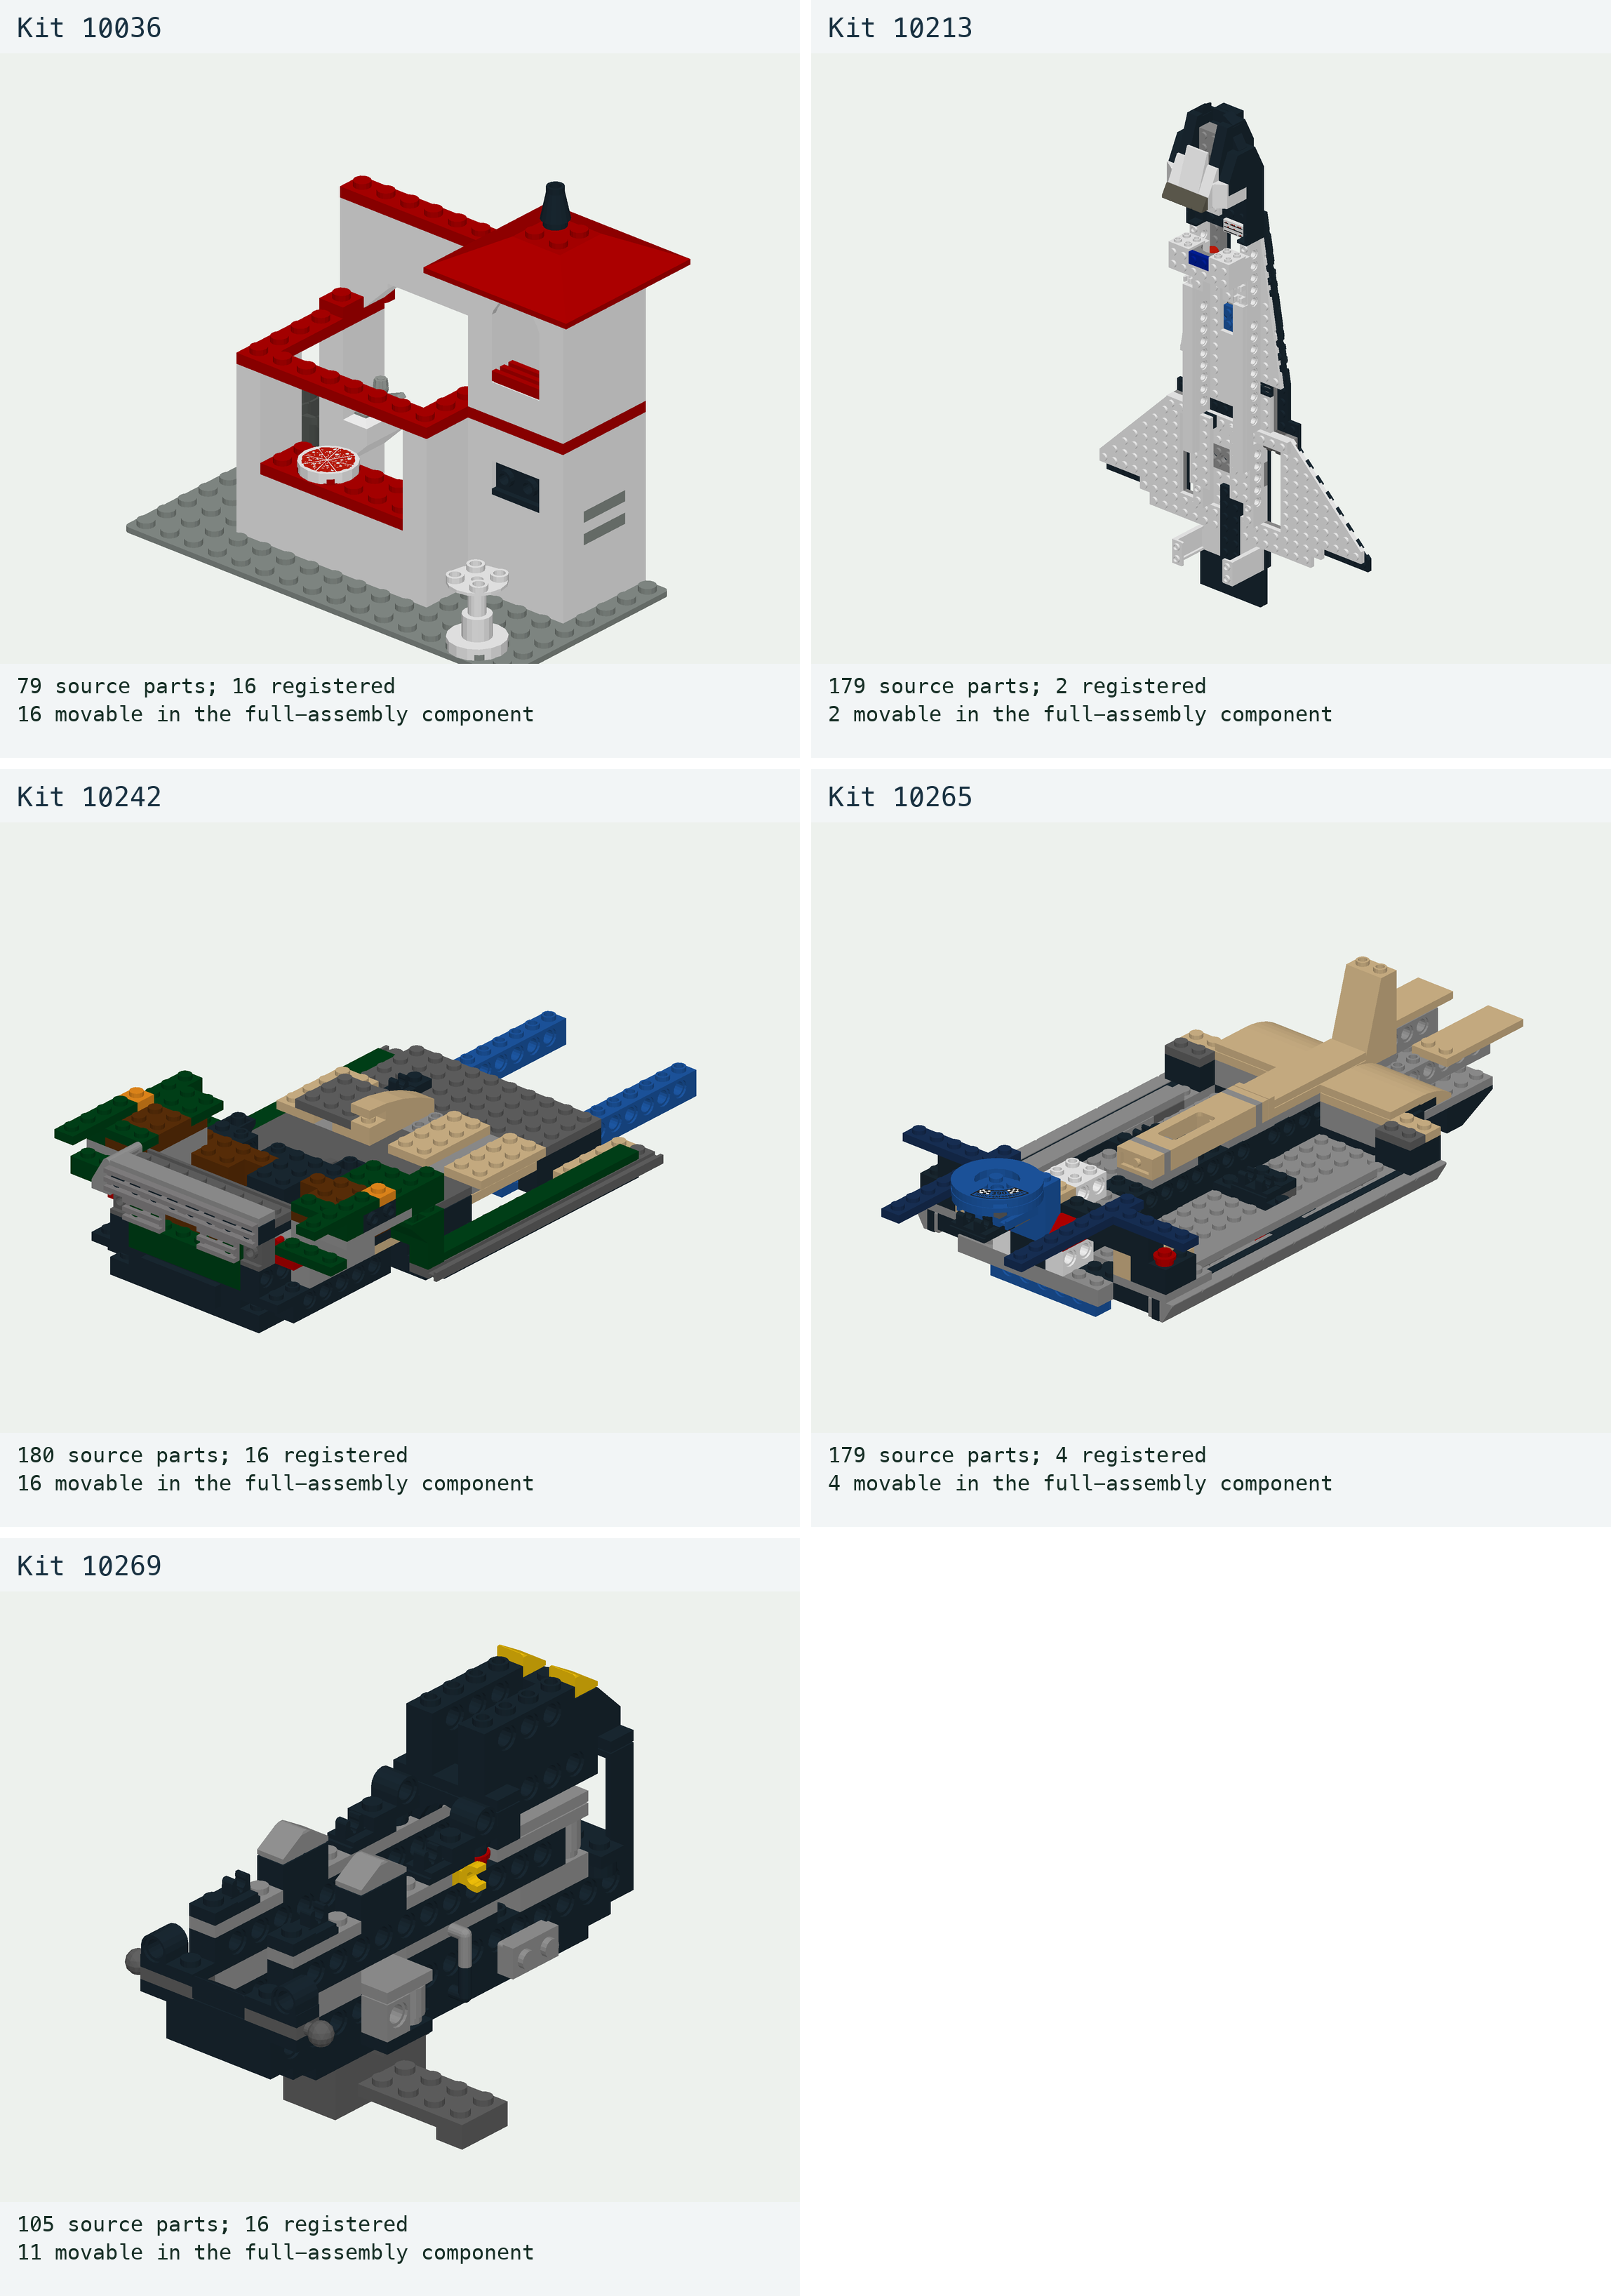
\includegraphics[width=.96\textwidth,height=.85\textheight,keepaspectratio]{figures/source-gallery-3.png}
\end{center}

\clearpage
\section{A certified optimal resource replay}
\begin{center}
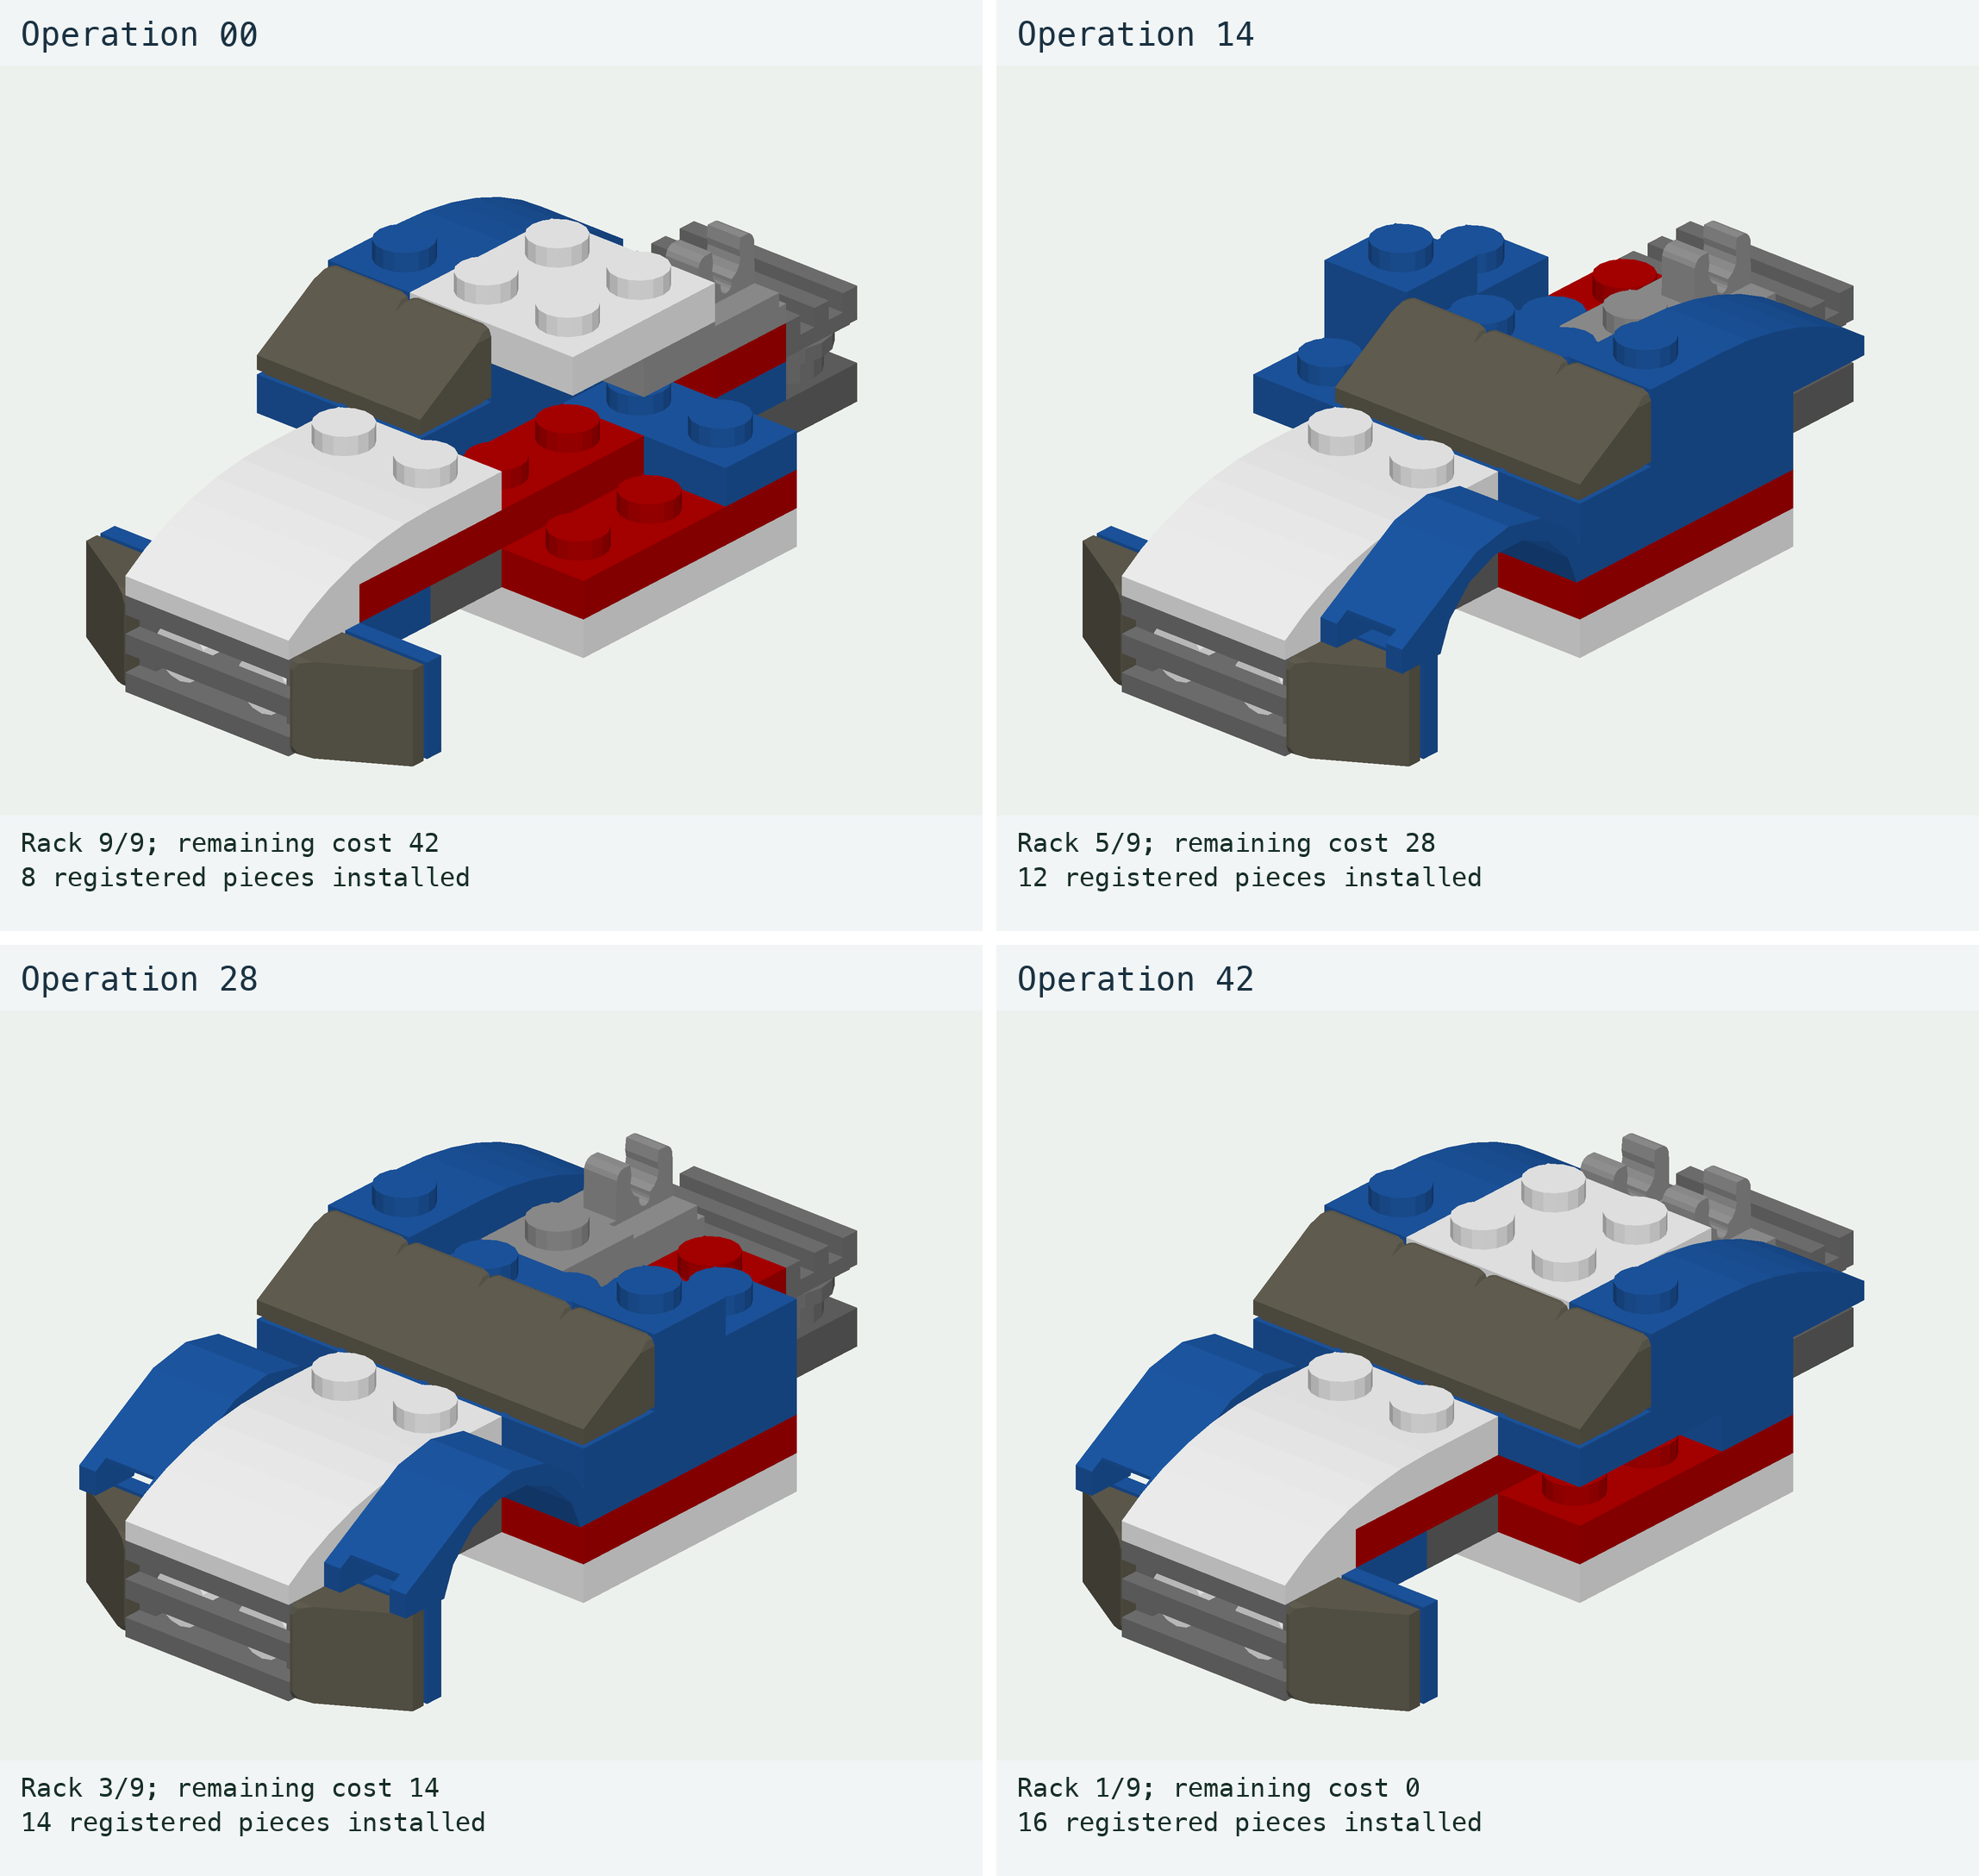
\includegraphics[width=.94\textwidth,height=.76\textheight,keepaspectratio]{figures/resource-replay.png}
\end{center}
This is an exact software-oracle witness, not a VLM trajectory.
All displayed states preserve source poses and certified connectivity.
The figure provenance contains the task ID, seed, occupancy, ledger,
step indices, and exact remaining cost. Rack holders and off-assembly
work are explicit abstractions of the task.

\clearpage
\section{Complete episode census}
``Jobs'' is the declared inspection count, ``Done'' its initially
completed subset, and A* expansions use seed 0 with the closure bound.
D1--D4 are length bins. Internal IDs are evaluator documentation;
participant IDs are consistently permuted by seed. Exact starts, goals,
jobs, witnesses, and oracle paths are available in the task bank.
\small
\begin{longtable}{llrrrrrr}
\toprule Episode & Tier & Rack & Jobs & Done & $C^*$ & $h$ & A* exp.\\\midrule\endhead
roadster-body-01 & D3 & 17 & 0 & 0 & 17 & 17 & 17\\
roadster-body-02 & D4 & 17 & 0 & 0 & 32 & 32 & 32\\
roadster-body-03 & D4 & 9 & 0 & 0 & 27 & 23 & 33\\
roadster-body-04 & D4 & 9 & 0 & 0 & 27 & 23 & 38\\
roadster-body-05 & D4 & 9 & 0 & 0 & 42 & 24 & 2555\\
roadster-body-06 & D4 & 9 & 0 & 0 & 42 & 24 & 2555\\
roadster-body-07 & D4 & 9 & 2 & 0 & 37 & 27 & 2185\\
roadster-body-08 & D4 & 9 & 2 & 0 & 37 & 27 & 2139\\
roadster-body-09 & D3 & 9 & 2 & 1 & 20 & 20 & 21\\
roadster-body-10 & D3 & 9 & 2 & 1 & 18 & 18 & 18\\
roadster-body-11 & D3 & 9 & 1 & 0 & 18 & 18 & 18\\
roadster-body-12 & D3 & 9 & 1 & 0 & 18 & 18 & 18\\
roadster-body-13 & D4 & 9 & 4 & 0 & 39 & 29 & 2131\\
roadster-body-14 & D4 & 9 & 4 & 0 & 39 & 29 & 2129\\
kart-deck-01 & D3 & 18 & 0 & 0 & 18 & 18 & 18\\
kart-deck-02 & D4 & 18 & 0 & 0 & 25 & 25 & 25\\
kart-deck-03 & D3 & 5 & 0 & 0 & 17 & 11 & 32\\
kart-deck-04 & D3 & 5 & 0 & 0 & 17 & 11 & 32\\
kart-deck-05 & D4 & 5 & 0 & 0 & 26 & 18 & 119\\
kart-deck-06 & D3 & 5 & 0 & 0 & 24 & 16 & 90\\
kart-deck-07 & D4 & 5 & 2 & 0 & 31 & 21 & 121\\
kart-deck-08 & D4 & 5 & 2 & 0 & 29 & 21 & 218\\
kart-deck-09 & D3 & 5 & 2 & 1 & 21 & 15 & 68\\
kart-deck-10 & D3 & 5 & 2 & 1 & 23 & 19 & 42\\
kart-deck-11 & D3 & 5 & 1 & 0 & 23 & 19 & 42\\
kart-deck-12 & D3 & 5 & 1 & 0 & 21 & 15 & 68\\
kart-deck-13 & D4 & 5 & 4 & 0 & 33 & 23 & 403\\
kart-deck-14 & D4 & 5 & 4 & 0 & 33 & 23 & 392\\
airframe-01 & D3 & 21 & 0 & 0 & 21 & 21 & 21\\
airframe-02 & D4 & 21 & 0 & 0 & 33 & 33 & 33\\
airframe-03 & D2 & 8 & 0 & 0 & 16 & 14 & 16\\
airframe-04 & D2 & 8 & 0 & 0 & 16 & 14 & 16\\
airframe-05 & D3 & 8 & 0 & 0 & 17 & 13 & 30\\
airframe-06 & D3 & 8 & 0 & 0 & 17 & 13 & 30\\
airframe-07 & D3 & 8 & 2 & 0 & 22 & 20 & 22\\
airframe-08 & D3 & 8 & 2 & 0 & 22 & 20 & 22\\
airframe-09 & D2 & 8 & 2 & 1 & 9 & 9 & 9\\
airframe-10 & D2 & 8 & 2 & 1 & 9 & 9 & 9\\
airframe-11 & D2 & 8 & 1 & 0 & 9 & 9 & 9\\
airframe-12 & D2 & 8 & 1 & 0 & 9 & 9 & 9\\
airframe-13 & D4 & 8 & 4 & 0 & 26 & 24 & 26\\
airframe-14 & D4 & 8 & 4 & 0 & 26 & 24 & 26\\
truck-cab-01 & D3 & 18 & 0 & 0 & 18 & 18 & 18\\
truck-cab-02 & D4 & 18 & 0 & 0 & 27 & 27 & 27\\
truck-cab-03 & D4 & 12 & 2 & 0 & 40 & 34 & 1522\\
truck-cab-04 & D4 & 12 & 2 & 0 & 36 & 30 & 809\\
truck-cab-05 & D3 & 12 & 2 & 1 & 21 & 19 & 22\\
truck-cab-06 & D3 & 12 & 2 & 1 & 21 & 19 & 22\\
truck-cab-07 & D3 & 12 & 1 & 0 & 21 & 19 & 22\\
truck-cab-08 & D3 & 12 & 1 & 0 & 21 & 19 & 22\\
truck-cab-09 & D4 & 12 & 4 & 0 & 42 & 36 & 1546\\
truck-cab-10 & D4 & 12 & 4 & 0 & 38 & 32 & 831\\
house-roof-01 & D3 & 18 & 0 & 0 & 18 & 18 & 18\\
house-roof-02 & D3 & 18 & 0 & 0 & 22 & 22 & 22\\
house-roof-03 & D3 & 5 & 0 & 0 & 21 & 17 & 37\\
house-roof-04 & D3 & 5 & 0 & 0 & 21 & 17 & 37\\
house-roof-05 & D3 & 5 & 0 & 0 & 22 & 18 & 45\\
house-roof-06 & D3 & 5 & 0 & 0 & 22 & 18 & 45\\
house-roof-07 & D4 & 5 & 2 & 0 & 27 & 23 & 54\\
house-roof-08 & D4 & 5 & 2 & 0 & 27 & 23 & 50\\
house-roof-09 & D3 & 5 & 2 & 1 & 17 & 17 & 19\\
house-roof-10 & D3 & 5 & 2 & 1 & 17 & 17 & 23\\
house-roof-11 & D3 & 5 & 1 & 0 & 17 & 17 & 23\\
house-roof-12 & D3 & 5 & 1 & 0 & 17 & 17 & 19\\
house-roof-13 & D4 & 5 & 4 & 0 & 33 & 29 & 76\\
house-roof-14 & D4 & 5 & 4 & 0 & 31 & 27 & 68\\
sports-body-01 & D2 & 22 & 0 & 0 & 10 & 10 & 10\\
sports-body-02 & D2 & 22 & 0 & 0 & 11 & 11 & 11\\
sports-body-03 & D3 & 8 & 2 & 0 & 17 & 17 & 17\\
source-10001-01 & D1 & 2 & 0 & 0 & 2 & 2 & 2\\
source-10001-02 & D1 & 2 & 0 & 0 & 1 & 1 & 1\\
source-10001-03 & D1 & 2 & 2 & 0 & 5 & 5 & 5\\
source-10001-04 & D1 & 2 & 2 & 0 & 6 & 6 & 6\\
source-10001-05 & D1 & 2 & 0 & 0 & 2 & 2 & 2\\
source-10001-06 & D1 & 2 & 0 & 0 & 1 & 1 & 1\\
source-10001-07 & D1 & 2 & 2 & 0 & 4 & 4 & 4\\
source-10001-08 & D1 & 2 & 2 & 0 & 4 & 4 & 4\\
source-10159-01 & D2 & 10 & 0 & 0 & 11 & 11 & 11\\
source-10159-02 & D2 & 10 & 0 & 0 & 9 & 9 & 9\\
source-10159-03 & D2 & 10 & 2 & 0 & 12 & 12 & 12\\
source-10159-04 & D2 & 10 & 2 & 0 & 11 & 11 & 11\\
source-10159-05 & D3 & 10 & 4 & 0 & 21 & 21 & 21\\
source-10159-06 & D2 & 10 & 4 & 0 & 14 & 14 & 14\\
source-10159-07 & D2 & 10 & 0 & 0 & 10 & 10 & 10\\
source-10159-08 & D2 & 10 & 0 & 0 & 14 & 12 & 45\\
source-10159-09 & D2 & 10 & 2 & 0 & 14 & 14 & 14\\
source-10159-10 & D2 & 10 & 2 & 0 & 9 & 9 & 9\\
source-10159-11 & D2 & 10 & 4 & 0 & 12 & 12 & 12\\
source-10159-12 & D2 & 10 & 4 & 0 & 16 & 16 & 16\\
source-10220-01 & D1 & 10 & 0 & 0 & 8 & 8 & 8\\
source-10220-02 & D1 & 10 & 0 & 0 & 7 & 7 & 7\\
source-10220-03 & D2 & 10 & 2 & 0 & 14 & 14 & 14\\
source-10220-04 & D2 & 10 & 2 & 0 & 13 & 13 & 13\\
source-10220-05 & D2 & 10 & 4 & 0 & 14 & 14 & 14\\
source-10220-06 & D3 & 10 & 4 & 0 & 19 & 19 & 19\\
source-10220-07 & D1 & 10 & 0 & 0 & 7 & 7 & 7\\
source-10220-08 & D2 & 10 & 0 & 0 & 11 & 11 & 11\\
source-10220-09 & D2 & 10 & 2 & 0 & 12 & 12 & 12\\
source-10220-10 & D2 & 10 & 2 & 0 & 10 & 10 & 10\\
source-10220-11 & D2 & 10 & 4 & 0 & 14 & 14 & 14\\
source-10220-12 & D2 & 10 & 4 & 0 & 14 & 14 & 14\\
source-10014-01 & D2 & 10 & 0 & 0 & 10 & 10 & 10\\
source-10014-02 & D3 & 10 & 0 & 0 & 21 & 21 & 22\\
source-10014-03 & D2 & 10 & 2 & 0 & 10 & 10 & 10\\
source-10014-04 & D3 & 10 & 2 & 0 & 20 & 20 & 20\\
source-10014-05 & D4 & 10 & 4 & 0 & 26 & 26 & 29\\
source-10014-06 & D3 & 10 & 4 & 0 & 21 & 21 & 21\\
source-10014-07 & D1 & 10 & 0 & 0 & 8 & 8 & 8\\
source-10014-08 & D2 & 10 & 0 & 0 & 15 & 15 & 15\\
source-10014-09 & D2 & 10 & 2 & 0 & 14 & 12 & 58\\
source-10014-10 & D2 & 10 & 2 & 0 & 14 & 14 & 15\\
source-10014-11 & D3 & 10 & 4 & 0 & 21 & 17 & 4372\\
source-10014-12 & D2 & 10 & 4 & 0 & 15 & 13 & 52\\
source-10128-01 & D1 & 10 & 0 & 0 & 5 & 5 & 5\\
source-10128-02 & D2 & 10 & 0 & 0 & 14 & 14 & 14\\
source-10128-03 & D2 & 10 & 2 & 0 & 15 & 15 & 15\\
source-10128-04 & D3 & 10 & 2 & 0 & 18 & 18 & 18\\
source-10128-05 & D3 & 10 & 4 & 0 & 24 & 24 & 24\\
source-10128-06 & D3 & 10 & 4 & 0 & 18 & 18 & 18\\
source-10128-07 & D2 & 10 & 0 & 0 & 10 & 10 & 10\\
source-10128-08 & D1 & 10 & 0 & 0 & 8 & 8 & 8\\
source-10128-09 & D2 & 10 & 2 & 0 & 11 & 11 & 11\\
source-10128-10 & D2 & 10 & 2 & 0 & 14 & 14 & 22\\
source-10128-11 & D2 & 10 & 4 & 0 & 15 & 15 & 15\\
source-10128-12 & D3 & 10 & 4 & 0 & 19 & 19 & 19\\
source-omr-31031-01 & D2 & 8 & 0 & 0 & 12 & 12 & 12\\
source-omr-31031-02 & D1 & 8 & 0 & 0 & 6 & 6 & 6\\
source-omr-31031-03 & D2 & 8 & 2 & 0 & 13 & 13 & 13\\
source-omr-31031-04 & D2 & 8 & 2 & 0 & 11 & 11 & 11\\
source-omr-31031-05 & D3 & 8 & 4 & 0 & 17 & 17 & 17\\
source-omr-31031-06 & D3 & 8 & 4 & 0 & 20 & 20 & 20\\
source-omr-31031-07 & D2 & 8 & 0 & 0 & 13 & 11 & 26\\
source-omr-31031-08 & D2 & 8 & 0 & 0 & 15 & 15 & 23\\
source-omr-31031-09 & D1 & 8 & 2 & 0 & 8 & 8 & 8\\
source-omr-31031-10 & D2 & 8 & 2 & 0 & 10 & 10 & 10\\
source-omr-31031-11 & D2 & 8 & 4 & 0 & 14 & 14 & 14\\
source-omr-31031-12 & D2 & 8 & 4 & 0 & 15 & 15 & 15\\
roadster-body-context-0-01 & D4 & 9 & 1 & 0 & 34 & 32 & 954\\
roadster-body-context-1-01 & D4 & 9 & 1 & 0 & 34 & 32 & 953\\
roadster-body-context-0-02 & D4 & 9 & 1 & 0 & 34 & 30 & 1018\\
roadster-body-context-1-02 & D4 & 9 & 1 & 0 & 34 & 30 & 1017\\
roadster-body-context-0-03 & D4 & 9 & 1 & 0 & 34 & 30 & 847\\
roadster-body-context-1-03 & D4 & 9 & 1 & 0 & 34 & 30 & 846\\
roadster-body-context-0-04 & D4 & 9 & 1 & 0 & 32 & 30 & 414\\
roadster-body-context-1-04 & D4 & 9 & 1 & 0 & 32 & 30 & 413\\
source-10036-01 & D2 & 10 & 0 & 0 & 16 & 16 & 16\\
source-10036-02 & D1 & 10 & 0 & 0 & 8 & 8 & 8\\
source-10036-03 & D2 & 10 & 0 & 0 & 12 & 12 & 12\\
source-10036-04 & D4 & 10 & 0 & 0 & 29 & 23 & 406\\
source-10036-05 & D2 & 10 & 2 & 0 & 16 & 16 & 16\\
source-10036-06 & D3 & 10 & 2 & 0 & 17 & 17 & 17\\
source-10036-07 & D3 & 10 & 2 & 0 & 17 & 17 & 17\\
source-10036-08 & D2 & 10 & 2 & 0 & 15 & 15 & 15\\
source-10036-09 & D4 & 10 & 4 & 0 & 27 & 27 & 27\\
source-10036-10 & D3 & 10 & 4 & 0 & 24 & 24 & 24\\
source-10036-11 & D4 & 10 & 4 & 0 & 26 & 26 & 26\\
source-10036-12 & D4 & 10 & 4 & 0 & 34 & 28 & 7595\\
source-10036-13 & D2 & 10 & 0 & 0 & 11 & 11 & 11\\
source-10036-14 & D2 & 10 & 0 & 0 & 10 & 10 & 10\\
source-10036-15 & D2 & 10 & 0 & 0 & 15 & 15 & 27\\
source-10036-16 & D2 & 10 & 0 & 0 & 12 & 12 & 12\\
source-10036-17 & D2 & 10 & 2 & 0 & 16 & 16 & 22\\
source-10036-18 & D4 & 10 & 2 & 0 & 26 & 16 & 3168\\
source-10036-19 & D3 & 10 & 2 & 0 & 24 & 14 & 2226\\
source-10036-20 & D2 & 10 & 2 & 0 & 14 & 14 & 21\\
source-10036-21 & D4 & 10 & 4 & 0 & 30 & 20 & 12578\\
source-10036-22 & D3 & 10 & 4 & 0 & 24 & 18 & 1714\\
source-10036-23 & D3 & 10 & 4 & 0 & 19 & 19 & 27\\
source-10036-24 & D3 & 10 & 4 & 0 & 20 & 20 & 56\\
source-10036-25 & D2 & 10 & 0 & 0 & 10 & 10 & 10\\
source-10036-26 & D1 & 10 & 0 & 0 & 6 & 6 & 6\\
source-10036-27 & D2 & 10 & 0 & 0 & 16 & 16 & 16\\
source-10036-28 & D2 & 10 & 0 & 0 & 9 & 9 & 9\\
source-10036-29 & D2 & 10 & 2 & 0 & 13 & 13 & 13\\
source-10036-30 & D2 & 10 & 2 & 0 & 13 & 13 & 13\\
source-10036-31 & D2 & 10 & 2 & 0 & 12 & 12 & 12\\
source-10036-32 & D2 & 10 & 2 & 0 & 13 & 11 & 14\\
source-10036-33 & D3 & 10 & 4 & 0 & 20 & 20 & 20\\
source-10036-34 & D3 & 10 & 4 & 0 & 22 & 22 & 22\\
source-10036-35 & D3 & 10 & 4 & 0 & 22 & 18 & 134\\
source-10036-36 & D3 & 10 & 4 & 0 & 22 & 22 & 22\\
source-10036-37 & D2 & 10 & 0 & 0 & 14 & 12 & 60\\
source-10036-38 & D4 & 10 & 0 & 0 & 27 & 17 & 786\\
source-10036-39 & D3 & 10 & 0 & 0 & 20 & 14 & 264\\
source-10036-40 & D1 & 10 & 0 & 0 & 5 & 5 & 7\\
source-10036-41 & D4 & 10 & 2 & 0 & 33 & 15 & 4640\\
source-10036-42 & D3 & 10 & 2 & 0 & 17 & 11 & 282\\
source-10036-43 & D2 & 10 & 2 & 0 & 14 & 12 & 101\\
source-10036-44 & D3 & 10 & 2 & 0 & 19 & 17 & 236\\
source-10036-45 & D3 & 10 & 4 & 0 & 19 & 15 & 726\\
source-10036-46 & D2 & 10 & 4 & 0 & 15 & 13 & 151\\
source-10036-47 & D4 & 10 & 4 & 0 & 32 & 22 & 11933\\
source-10036-48 & D2 & 10 & 4 & 0 & 14 & 10 & 311\\
source-10213-01 & D1 & 2 & 0 & 0 & 2 & 2 & 2\\
source-10213-02 & D1 & 2 & 0 & 0 & 1 & 1 & 1\\
source-10213-03 & D1 & 2 & 0 & 0 & 1 & 1 & 1\\
source-10213-04 & D1 & 2 & 2 & 0 & 6 & 6 & 6\\
source-10213-05 & D1 & 2 & 2 & 0 & 4 & 4 & 4\\
source-10213-06 & D1 & 2 & 2 & 0 & 5 & 5 & 5\\
source-10213-07 & D1 & 2 & 2 & 0 & 5 & 5 & 5\\
source-10213-08 & D1 & 2 & 0 & 0 & 2 & 2 & 2\\
source-10213-09 & D1 & 2 & 0 & 0 & 1 & 1 & 1\\
source-10213-10 & D1 & 2 & 0 & 0 & 1 & 1 & 1\\
source-10213-11 & D1 & 2 & 2 & 0 & 4 & 4 & 4\\
source-10213-12 & D1 & 2 & 2 & 0 & 2 & 2 & 2\\
source-10213-13 & D1 & 2 & 2 & 0 & 3 & 3 & 3\\
source-10213-14 & D1 & 2 & 2 & 0 & 3 & 3 & 3\\
source-10213-15 & D1 & 2 & 0 & 0 & 1 & 1 & 1\\
source-10213-16 & D1 & 2 & 0 & 0 & 2 & 2 & 2\\
source-10213-17 & D1 & 2 & 0 & 0 & 1 & 1 & 1\\
source-10213-18 & D1 & 2 & 2 & 0 & 4 & 4 & 4\\
source-10213-19 & D1 & 2 & 2 & 0 & 5 & 5 & 5\\
source-10213-20 & D1 & 2 & 2 & 0 & 4 & 4 & 4\\
source-10213-21 & D1 & 2 & 2 & 0 & 3 & 3 & 3\\
source-10213-22 & D1 & 2 & 0 & 0 & 1 & 1 & 1\\
source-10213-23 & D1 & 2 & 0 & 0 & 1 & 1 & 1\\
source-10213-24 & D1 & 2 & 0 & 0 & 2 & 2 & 2\\
source-10213-25 & D1 & 2 & 2 & 0 & 3 & 3 & 3\\
source-10213-26 & D1 & 2 & 2 & 0 & 4 & 4 & 4\\
source-10213-27 & D1 & 2 & 2 & 0 & 5 & 5 & 5\\
source-10213-28 & D1 & 2 & 2 & 0 & 4 & 4 & 4\\
source-omr-10242-01 & D1 & 10 & 0 & 0 & 8 & 8 & 8\\
source-omr-10242-02 & D2 & 10 & 0 & 0 & 14 & 14 & 14\\
source-omr-10242-03 & D1 & 10 & 0 & 0 & 7 & 7 & 7\\
source-omr-10242-04 & D2 & 10 & 0 & 0 & 11 & 11 & 11\\
source-omr-10242-05 & D2 & 10 & 2 & 0 & 13 & 13 & 13\\
source-omr-10242-06 & D2 & 10 & 2 & 0 & 16 & 16 & 16\\
source-omr-10242-07 & D2 & 10 & 2 & 0 & 11 & 11 & 11\\
source-omr-10242-08 & D2 & 10 & 2 & 0 & 15 & 15 & 15\\
source-omr-10242-09 & D3 & 10 & 4 & 0 & 17 & 17 & 17\\
source-omr-10242-10 & D2 & 10 & 4 & 0 & 16 & 16 & 16\\
source-omr-10242-11 & D2 & 10 & 4 & 0 & 14 & 14 & 14\\
source-omr-10242-12 & D3 & 10 & 4 & 0 & 17 & 17 & 17\\
source-omr-10242-13 & D2 & 10 & 0 & 0 & 9 & 9 & 9\\
source-omr-10242-14 & D1 & 10 & 0 & 0 & 7 & 7 & 7\\
source-omr-10242-15 & D2 & 10 & 0 & 0 & 9 & 9 & 9\\
source-omr-10242-16 & D1 & 10 & 0 & 0 & 8 & 8 & 8\\
source-omr-10242-17 & D2 & 10 & 2 & 0 & 13 & 13 & 13\\
source-omr-10242-18 & D2 & 10 & 2 & 0 & 16 & 16 & 16\\
source-omr-10242-19 & D2 & 10 & 2 & 0 & 12 & 12 & 12\\
source-omr-10242-20 & D2 & 10 & 2 & 0 & 12 & 12 & 12\\
source-omr-10242-21 & D2 & 10 & 4 & 0 & 14 & 14 & 14\\
source-omr-10242-22 & D2 & 10 & 4 & 0 & 13 & 13 & 13\\
source-omr-10242-23 & D2 & 10 & 4 & 0 & 13 & 13 & 13\\
source-omr-10242-24 & D2 & 10 & 4 & 0 & 15 & 15 & 15\\
source-omr-10242-25 & D2 & 10 & 0 & 0 & 11 & 11 & 11\\
source-omr-10242-26 & D1 & 10 & 0 & 0 & 7 & 7 & 7\\
source-omr-10242-27 & D1 & 10 & 0 & 0 & 6 & 6 & 6\\
source-omr-10242-28 & D2 & 10 & 0 & 0 & 10 & 10 & 10\\
source-omr-10242-29 & D2 & 10 & 2 & 0 & 9 & 9 & 9\\
source-omr-10242-30 & D3 & 10 & 2 & 0 & 17 & 17 & 17\\
source-omr-10242-31 & D2 & 10 & 2 & 0 & 10 & 10 & 10\\
source-omr-10242-32 & D2 & 10 & 2 & 0 & 12 & 12 & 12\\
source-omr-10242-33 & D2 & 10 & 4 & 0 & 14 & 14 & 14\\
source-omr-10242-34 & D2 & 10 & 4 & 0 & 14 & 14 & 14\\
source-omr-10242-35 & D2 & 10 & 4 & 0 & 15 & 15 & 15\\
source-omr-10242-36 & D2 & 10 & 4 & 0 & 14 & 14 & 14\\
source-omr-10242-37 & D2 & 10 & 0 & 0 & 10 & 10 & 10\\
source-omr-10242-38 & D1 & 10 & 0 & 0 & 8 & 8 & 8\\
source-omr-10242-39 & D1 & 10 & 0 & 0 & 7 & 7 & 7\\
source-omr-10242-40 & D1 & 10 & 0 & 0 & 8 & 8 & 8\\
source-omr-10242-41 & D2 & 10 & 2 & 0 & 10 & 10 & 10\\
source-omr-10242-42 & D2 & 10 & 2 & 0 & 11 & 11 & 11\\
source-omr-10242-43 & D2 & 10 & 2 & 0 & 11 & 11 & 11\\
source-omr-10242-44 & D2 & 10 & 2 & 0 & 12 & 12 & 12\\
source-omr-10242-45 & D2 & 10 & 4 & 0 & 16 & 16 & 16\\
source-omr-10242-46 & D3 & 10 & 4 & 0 & 17 & 17 & 17\\
source-omr-10242-47 & D3 & 10 & 4 & 0 & 17 & 17 & 17\\
source-omr-10242-48 & D3 & 10 & 4 & 0 & 18 & 18 & 18\\
source-omr-10265-01 & D1 & 3 & 0 & 0 & 2 & 2 & 2\\
source-omr-10265-02 & D1 & 3 & 0 & 0 & 1 & 1 & 1\\
source-omr-10265-03 & D1 & 3 & 0 & 0 & 1 & 1 & 1\\
source-omr-10265-04 & D1 & 3 & 0 & 0 & 3 & 3 & 3\\
source-omr-10265-05 & D1 & 3 & 2 & 0 & 5 & 5 & 5\\
source-omr-10265-06 & D1 & 3 & 2 & 0 & 7 & 7 & 7\\
source-omr-10265-07 & D1 & 3 & 2 & 0 & 4 & 4 & 4\\
source-omr-10265-08 & D1 & 3 & 2 & 0 & 5 & 5 & 5\\
source-omr-10265-09 & D2 & 3 & 4 & 0 & 9 & 9 & 9\\
source-omr-10265-10 & D2 & 3 & 4 & 0 & 10 & 10 & 10\\
source-omr-10265-11 & D2 & 3 & 4 & 0 & 12 & 12 & 12\\
source-omr-10265-12 & D2 & 3 & 4 & 0 & 9 & 9 & 9\\
source-omr-10265-13 & D1 & 3 & 0 & 0 & 2 & 2 & 2\\
source-omr-10265-14 & D1 & 3 & 0 & 0 & 2 & 2 & 2\\
source-omr-10265-15 & D1 & 3 & 0 & 0 & 2 & 2 & 2\\
source-omr-10265-16 & D1 & 3 & 0 & 0 & 1 & 1 & 1\\
source-omr-10265-17 & D1 & 3 & 2 & 0 & 4 & 4 & 4\\
source-omr-10265-18 & D1 & 3 & 2 & 0 & 7 & 7 & 7\\
source-omr-10265-19 & D1 & 3 & 2 & 0 & 5 & 5 & 5\\
source-omr-10265-20 & D1 & 3 & 2 & 0 & 5 & 5 & 5\\
source-omr-10265-21 & D2 & 3 & 4 & 0 & 9 & 9 & 9\\
source-omr-10265-22 & D2 & 3 & 4 & 0 & 9 & 9 & 9\\
source-omr-10265-23 & D2 & 3 & 4 & 0 & 9 & 9 & 9\\
source-omr-10265-24 & D2 & 3 & 4 & 0 & 9 & 9 & 9\\
source-omr-10265-25 & D1 & 3 & 0 & 0 & 2 & 2 & 2\\
source-omr-10265-26 & D1 & 3 & 0 & 0 & 3 & 3 & 3\\
source-omr-10265-27 & D1 & 3 & 0 & 0 & 3 & 3 & 3\\
source-omr-10265-28 & D1 & 3 & 0 & 0 & 2 & 2 & 2\\
source-omr-10265-29 & D1 & 3 & 2 & 0 & 3 & 3 & 3\\
source-omr-10265-30 & D1 & 3 & 2 & 0 & 4 & 4 & 4\\
source-omr-10265-31 & D1 & 3 & 2 & 0 & 5 & 5 & 5\\
source-omr-10265-32 & D1 & 3 & 2 & 0 & 5 & 5 & 5\\
source-omr-10265-33 & D1 & 3 & 4 & 0 & 7 & 7 & 7\\
source-omr-10265-34 & D1 & 3 & 4 & 0 & 7 & 7 & 7\\
source-omr-10265-35 & D1 & 3 & 4 & 0 & 7 & 7 & 7\\
source-omr-10265-36 & D1 & 3 & 4 & 0 & 8 & 8 & 8\\
source-omr-10265-37 & D1 & 3 & 0 & 0 & 2 & 2 & 2\\
source-omr-10265-38 & D1 & 3 & 0 & 0 & 3 & 3 & 3\\
source-omr-10265-39 & D1 & 3 & 0 & 0 & 1 & 1 & 1\\
source-omr-10265-40 & D1 & 3 & 0 & 0 & 1 & 1 & 1\\
source-omr-10265-41 & D1 & 3 & 2 & 0 & 8 & 8 & 8\\
source-omr-10265-42 & D1 & 3 & 2 & 0 & 6 & 6 & 6\\
source-omr-10265-43 & D1 & 3 & 2 & 0 & 7 & 7 & 7\\
source-omr-10265-44 & D1 & 3 & 2 & 0 & 6 & 6 & 6\\
source-omr-10265-45 & D2 & 3 & 4 & 0 & 9 & 9 & 9\\
source-omr-10265-46 & D2 & 3 & 4 & 0 & 9 & 9 & 9\\
source-omr-10265-47 & D2 & 3 & 4 & 0 & 9 & 9 & 9\\
source-omr-10265-48 & D1 & 3 & 4 & 0 & 8 & 8 & 8\\
source-omr-10269-01 & D2 & 10 & 0 & 0 & 11 & 11 & 11\\
source-omr-10269-02 & D2 & 10 & 0 & 0 & 13 & 13 & 13\\
source-omr-10269-03 & D2 & 10 & 0 & 0 & 12 & 12 & 12\\
source-omr-10269-04 & D2 & 10 & 0 & 0 & 9 & 9 & 9\\
source-omr-10269-05 & D3 & 10 & 2 & 0 & 17 & 17 & 17\\
source-omr-10269-06 & D3 & 10 & 2 & 0 & 18 & 18 & 18\\
source-omr-10269-07 & D2 & 10 & 2 & 0 & 16 & 16 & 16\\
source-omr-10269-08 & D2 & 10 & 2 & 0 & 15 & 15 & 15\\
source-omr-10269-09 & D3 & 10 & 4 & 0 & 22 & 22 & 22\\
source-omr-10269-10 & D3 & 10 & 4 & 0 & 21 & 21 & 21\\
source-omr-10269-11 & D3 & 10 & 4 & 0 & 19 & 19 & 19\\
source-omr-10269-12 & D3 & 10 & 4 & 0 & 20 & 20 & 20\\
source-omr-10269-13 & D1 & 10 & 0 & 0 & 6 & 6 & 6\\
source-omr-10269-14 & D2 & 10 & 0 & 0 & 11 & 11 & 11\\
source-omr-10269-15 & D2 & 10 & 0 & 0 & 10 & 10 & 10\\
source-omr-10269-16 & D1 & 10 & 0 & 0 & 7 & 7 & 7\\
source-omr-10269-17 & D2 & 10 & 2 & 0 & 14 & 14 & 14\\
source-omr-10269-18 & D2 & 10 & 2 & 0 & 15 & 15 & 15\\
source-omr-10269-19 & D2 & 10 & 2 & 0 & 11 & 11 & 11\\
source-omr-10269-20 & D2 & 10 & 2 & 0 & 12 & 12 & 12\\
source-omr-10269-21 & D3 & 10 & 4 & 0 & 18 & 18 & 18\\
source-omr-10269-22 & D2 & 10 & 4 & 0 & 16 & 16 & 16\\
source-omr-10269-23 & D2 & 10 & 4 & 0 & 13 & 13 & 13\\
source-omr-10269-24 & D2 & 10 & 4 & 0 & 14 & 14 & 14\\
source-omr-10269-25 & D2 & 10 & 0 & 0 & 14 & 14 & 14\\
source-omr-10269-26 & D1 & 10 & 0 & 0 & 7 & 7 & 7\\
source-omr-10269-27 & D2 & 10 & 0 & 0 & 11 & 11 & 11\\
source-omr-10269-28 & D2 & 10 & 0 & 0 & 10 & 10 & 10\\
source-omr-10269-29 & D2 & 10 & 2 & 0 & 12 & 12 & 12\\
source-omr-10269-30 & D2 & 10 & 2 & 0 & 13 & 13 & 13\\
source-omr-10269-31 & D2 & 10 & 2 & 0 & 14 & 14 & 14\\
source-omr-10269-32 & D2 & 10 & 2 & 0 & 12 & 12 & 12\\
source-omr-10269-33 & D2 & 10 & 4 & 0 & 15 & 15 & 15\\
source-omr-10269-34 & D3 & 10 & 4 & 0 & 17 & 17 & 17\\
source-omr-10269-35 & D2 & 10 & 4 & 0 & 14 & 14 & 14\\
source-omr-10269-36 & D2 & 10 & 4 & 0 & 15 & 15 & 15\\
source-omr-10269-37 & D2 & 10 & 0 & 0 & 12 & 12 & 12\\
source-omr-10269-38 & D2 & 10 & 0 & 0 & 13 & 13 & 13\\
source-omr-10269-39 & D2 & 10 & 0 & 0 & 12 & 12 & 12\\
source-omr-10269-40 & D1 & 10 & 0 & 0 & 8 & 8 & 8\\
source-omr-10269-41 & D2 & 10 & 2 & 0 & 15 & 15 & 15\\
source-omr-10269-42 & D2 & 10 & 2 & 0 & 13 & 13 & 13\\
source-omr-10269-43 & D2 & 10 & 2 & 0 & 12 & 12 & 14\\
source-omr-10269-44 & D2 & 10 & 2 & 0 & 16 & 16 & 16\\
source-omr-10269-45 & D2 & 10 & 4 & 0 & 16 & 16 & 16\\
source-omr-10269-46 & D3 & 10 & 4 & 0 & 18 & 18 & 18\\
source-omr-10269-47 & D3 & 10 & 4 & 0 & 17 & 17 & 17\\
source-omr-10269-48 & D2 & 10 & 4 & 0 & 15 & 15 & 15\\
source-10014-context-0-01 & D3 & 10 & 1 & 0 & 18 & 18 & 23\\
source-10014-context-1-01 & D3 & 10 & 1 & 0 & 18 & 18 & 18\\
source-10014-context-0-02 & D3 & 10 & 1 & 0 & 22 & 22 & 31\\
source-10014-context-1-02 & D3 & 10 & 1 & 0 & 22 & 22 & 22\\
source-10036-context-0-01 & D2 & 10 & 0 & 0 & 15 & 15 & 15\\
source-10036-context-1-01 & D2 & 10 & 0 & 0 & 15 & 15 & 15\\
source-10036-context-0-02 & D2 & 10 & 0 & 0 & 16 & 16 & 16\\
source-10036-context-1-02 & D2 & 10 & 0 & 0 & 16 & 16 & 16\\
source-10036-intervention-2-context-0-01 & D3 & 10 & 0 & 0 & 17 & 17 & 17\\
source-10036-intervention-2-context-1-01 & D3 & 10 & 0 & 0 & 17 & 17 & 17\\
source-10036-intervention-2-context-0-02 & D2 & 10 & 0 & 0 & 15 & 15 & 15\\
source-10036-intervention-2-context-1-02 & D2 & 10 & 0 & 0 & 15 & 15 & 15\\
\bottomrule\end{longtable}

